\documentclass{beamer}
\usepackage[utf8]{inputenc}

\usetheme{Madrid}
\usecolortheme{default}
\usepackage{amsmath,amssymb,amsfonts,amsthm}
\usepackage{txfonts}
\usepackage{tkz-euclide}
\usepackage{listings}
\usepackage{adjustbox}
\usepackage{array}
\usepackage{tabularx}
\usepackage{gvv}
\usepackage{lmodern}
\usepackage{circuitikz}
\usepackage{tikz}
\usepackage{graphicx}

\setbeamertemplate{page number in head/foot}[totalframenumber]

\usepackage{tcolorbox}
\tcbuselibrary{minted,breakable,xparse,skins}



\definecolor{bg}{gray}{0.95}
\DeclareTCBListing{mintedbox}{O{}m!O{}}{%
  breakable=true,
  listing engine=minted,
  listing only,
  minted language=#2,
  minted style=default,
  minted options={%
    linenos,
    gobble=0,
    breaklines=true,
    breakafter=,,
    fontsize=\small,
    numbersep=8pt,
    #1},
  boxsep=0pt,
  left skip=0pt,
  right skip=0pt,
  left=25pt,
  right=0pt,
  top=3pt,
  bottom=3pt,
  arc=5pt,
  leftrule=0pt,
  rightrule=0pt,
  bottomrule=2pt,
  toprule=2pt,
  colback=bg,
  colframe=orange!70,
  enhanced,
  overlay={%
    \begin{tcbclipinterior}
    \fill[orange!20!white] (frame.south west) rectangle ([xshift=20pt]frame.north west);
    \end{tcbclipinterior}},
  #3,
}
\lstset{
    language=C,
    basicstyle=\ttfamily\small,
    keywordstyle=\color{blue},
    stringstyle=\color{orange},
    commentstyle=\color{green!60!black},
    numbers=left,
    numberstyle=\tiny\color{gray},
    breaklines=true,
    showstringspaces=false,
}
%------------------------------------------------------------
%This block of code defines the information to appear in the
%Title page
\title %optional
{1.9.19}
\date{August 31,2025}


\author 
{Josyula G S Avaneesh - EE25BTECH11030}



\begin{document}



\frame{\titlepage}
\begin{frame}{Question}
Find the value of $x$ for which the distance between the points $\vec{A}(x,2)$ and $\vec{B}(9,8)$ is $10$ units.
\end{frame}



\begin{frame}{Equation}

Distance between 2 vectors $\vec{A}$ and $\vec{B}$ can be represented as:
\begin{align}
    \norm{AB}=\sqrt{\brak{\vec{B}-\vec{A}}^T\brak{\vec{B}-\vec{A}}}
\end{align}
\end{frame}

\begin{frame}{Theoretical Solution}

Given details:
\begin{align}
    \vec{B}=\myvec{9\\8}\\  \vec{A}=\myvec{x\\2}\\ \norm{AB}=10 
\end{align}
\end{frame}

\begin{frame}{Theoretical Solution}

By substituting values:
\begin{align}
    \norm{AB}=\sqrt{\myvec{9-x & 8-2}\myvec{9-x \\8-2}}=\sqrt{\myvec{9-x & 6}\myvec{9-x \\6}}\\
    =\sqrt{(9-x)^2+ \brak{6}^2} =\sqrt{(x^2-18x+81)+36}=\sqrt{x^2-18x+117}
\end{align}

\end{frame}


\begin{frame}{Theoretical Solution}
Now from equation (3) and (4), we can say that :
\begin{align}
     \sqrt{x^2-18x+117}=10
\end{align}
Square on both sides
\begin{align}
   x^2 -18x+117&=100\\
    x^2-18x+17&=0\\
    \text{On solving this we get,}\
    x=1\  or\ x=17
\end{align}

\end{frame}
\begin{frame}{Theoretical Solution}
\textbf{Final answer:}\\
The values of $x$ are $1$ and $17$.
Therefore, the points $\vec{A}(x,2)$ are $(1,2) \ or \ (17,2)$.
\end{frame}

\begin{frame}[fragile]
    \frametitle{C Code (1) - Function to generate a line segment }

    \begin{lstlisting}

#include <math.h>

// Function to calculate distance between two points (x1,y1) and (x2,y2)
double distance(double x1, double y1, double x2, double y2) {
    double dx = x2 - x1;
    double dy = y2 - y1;
    return sqrt(dx * dx + dy * dy);
}

    \end{lstlisting}
\end{frame}


\begin{frame}[fragile]
    \frametitle{Python Code - Using Shared Object}
    \begin{lstlisting}

import ctypes
import numpy as np
import matplotlib.pyplot as plt
import matplotlib as mp
mp.use("TkAgg")

# Load shared object
lib = ctypes.CDLL("./line.so")

# Define function signature
lib.distance.argtypes = [ctypes.c_double, ctypes.c_double,
                         ctypes.c_double, ctypes.c_double]
lib.distance.restype = ctypes.c_double

   



\end{lstlisting}
\end{frame}

\begin{frame}[fragile]
    \frametitle{Python Code - Using Shared Object}
    \begin{lstlisting}
# Fixed point B
B = (9, 8)

# Two A points
A1 = (1, 2)
A2 = (17,2)

# Distances from B using C function
d1 = lib.distance(B[0], B[1], A1[0], A1[1])
d2 = lib.distance(B[0], B[1], A2[0], A2[1])
# Plot line segments B->A1 and B->A2
plt.figure(figsize=(6,6))

\end{lstlisting}
\end{frame}
\begin{frame}[fragile]
    \frametitle{Python Code - Using Shared Object}
    \begin{lstlisting}
# Line B->A1
plt.plot([B[0], A1[0]], [B[1], A1[1]], 'b-o', label=f"B→A1 {A1}, d={d1:.2f}")
plt.text(A1[0], A1[1], f"A1{A1}", fontsize=12, ha='left')

# Line B->A2
plt.plot([B[0], A2[0]], [B[1], A2[1]], 'g-o', label=f"B→A2 {A2}, d={d2:.2f}")
plt.text(A2[0], A2[1], f"A2{A2}", fontsize=12, ha='left')

# Mark B
plt.scatter(B[0], B[1], color='red')
plt.text(B[0], B[1], "B(9,8)", fontsize=12, ha='right')



\end{lstlisting}
\end{frame}
\begin{frame}[fragile]
    \frametitle{Python Code - Using Shared Object}
    \begin{lstlisting}
# Labels & styling
plt.xlabel("X-axis")
plt.ylabel("Y-axis")
plt.title("Line Segments from B(9,8) to A1 and A2")
plt.legend()
plt.grid(True)
plt.axis("equal")
plt.savefig('/home/avaneesh1/Matrix/ee1030-2025/ee25btech11030/matgeo/1.9.19/figs/distance.png')
plt.show(block=True)
\end{lstlisting}
\end{frame}


\begin{frame}{Plot-Using Both C and Python}
    \centering
    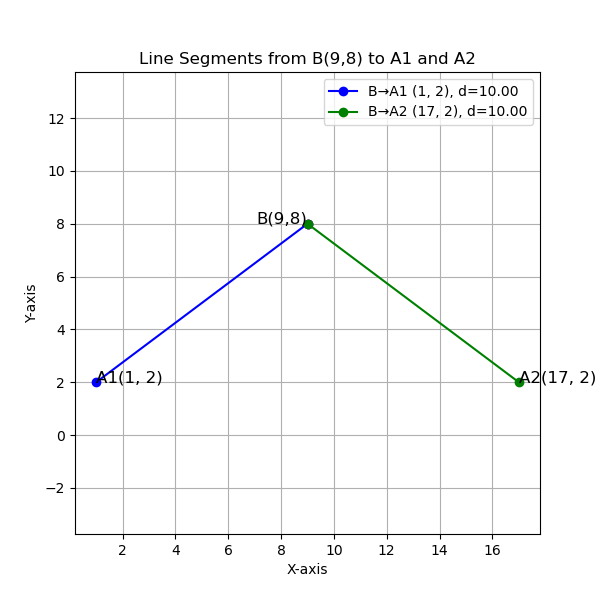
\includegraphics[width=\columnwidth, height=0.8\textheight, keepaspectratio]{figs/distance.png}     
\end{frame}

\begin{frame}[fragile]
    \frametitle{Python Code}
    \begin{lstlisting}
import numpy as np
import matplotlib.pyplot as plt
import matplotlib as mp
mp.use("TkAgg")

# Fixed point B
B = (9, 8)

# Two A points
A1 = (1, 2)
A2 = (17, 2)

# Distances using numpy
d1 = np.sqrt((A1[0]-B[0])**2 + (A1[1]-B[1])**2)
d2 = np.sqrt((A2[0]-B[0])**2 + (A2[1]-B[1])**2)



\end{lstlisting}
\end{frame}

\begin{frame}[fragile]
    \frametitle{Python Code }
    \begin{lstlisting}
# Plot line segments B->A1 and B->A2
plt.figure(figsize=(6,6))

# Line B->A1
plt.plot([B[0], A1[0]], [B[1], A1[1]], 'b-o', label=f"B→A1 {A1}, d={d1:.2f}")
plt.text(A1[0], A1[1], f"A1{A1}", fontsize=12, ha='left')

# Line B->A2
plt.plot([B[0], A2[0]], [B[1], A2[1]], 'g-o', label=f"B→A2 {A2}, d={d2:.2f}")
plt.text(A2[0], A2[1], f"A2{A2}", fontsize=12, ha='left')


\end{lstlisting}
\end{frame}

\begin{frame}[fragile]
    \frametitle{Python Code }
    \begin{lstlisting}
# Mark B
plt.scatter(B[0], B[1], color='red')
plt.text(B[0], B[1], "B(9,8)", fontsize=12, ha='right')

# Labels & styling
plt.xlabel("X-axis")
plt.ylabel("Y-axis")
plt.title("Line Segments from B(9,8) to A1 and A2")
plt.legend()
plt.grid(True)
plt.axis("equal")
plt.savefig('/home/avaneesh1/Matrix/ee1030-2025/ee25btech11030/matgeo/1.9.19/figs/distance2.png')
plt.show(block=True)

\end{lstlisting}
\end{frame}




\begin{frame}{Plot-Using only Python}
    \centering
    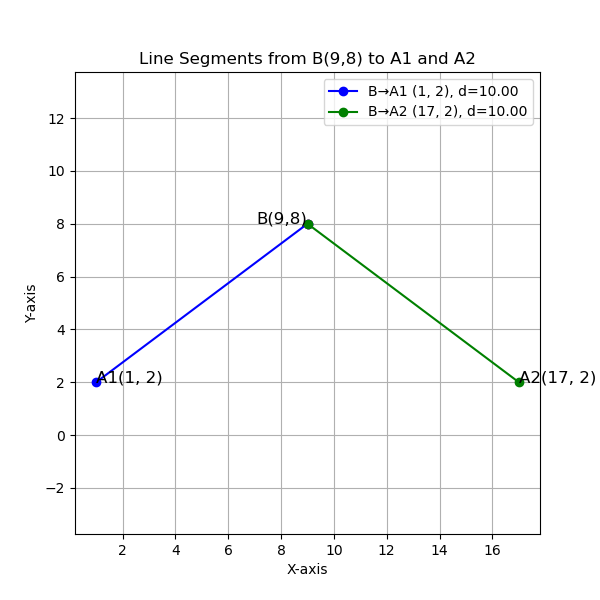
\includegraphics[width=\columnwidth, height=0.8\textheight, keepaspectratio]{figs/distance2.png}     
\end{frame}


\end{document}